\section{Resolução Questão 17}

\begin{frame}{Questão 17}
Considere um programa de TV em que um participante deve escolher uma de três portas. Atrás de uma das portas existe um carro, enquanto nada existe atrás das outras duas.

\vspace{0.3cm}
A produção coloca o prêmio de forma aleatória atrás de uma das portas. Após a escolha de uma porta, o apresentador abre uma das outras portas que não contém o prêmio, e pergunta ao participante se ele deseja trocar sua escolha.
\end{frame}

% Slide 2: Portas
\begin{frame}{Qual porta escolher?}
\centering
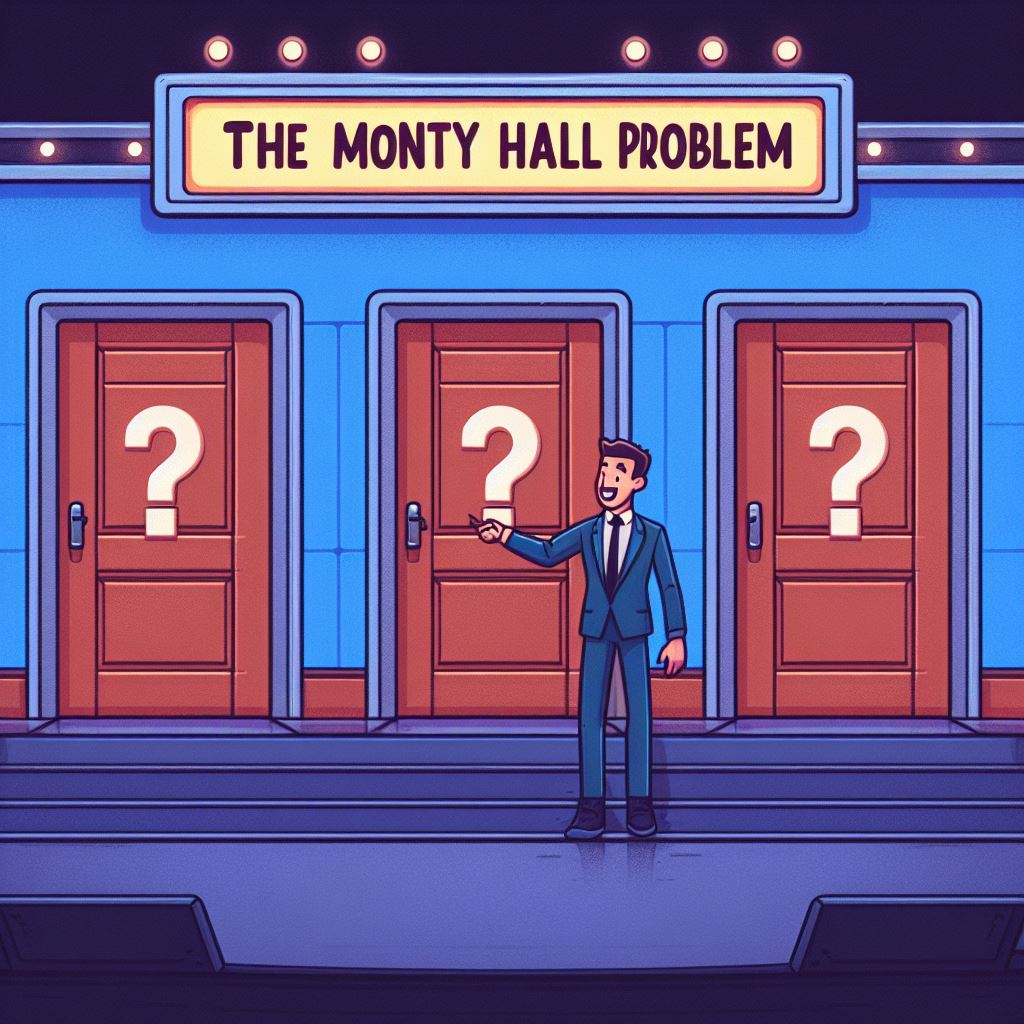
\includegraphics[width=0.45\textwidth]{figures/MontyHall.jpeg}
\end{frame}

% Slide 3: Código
\begin{frame}[fragile]{Simulação - Problema de Monty Hall}
\begin{lstlisting}
// --- Simulação do Problema de Monty Hall com Registro de Convergência ---

// 1. Definição dos parâmetros
num_simulacoes = 50000;
nome_arquivo = "monty_hall_convergence.csv";

// 2. Inicialização dos contadores e da matriz para armazenar os resultados
vitorias_mantendo = 0;
vitorias_trocando = 0;
resultados_convergencia = zeros(num_simulacoes, 3);

\end{lstlisting}
\end{frame}

\begin{frame}[fragile]{Simulação - Problema de Monty Hall}
\begin{lstlisting}
// 3. Loop principal da simulação
for i = 1:num_simulacoes
    porta_premiada = grand(1, 1, 'uin', 1, 3);      // Porta com o prêmio
    escolha_inicial = grand(1, 1, 'uin', 1, 3);     // Escolha do participante

    // Verifica se ganharíamos mantendo ou trocando a escolha
    if escolha_inicial == porta_premiada then
        vitorias_mantendo = vitorias_mantendo + 1;
    else
        vitorias_trocando = vitorias_trocando + 1;
    end

\end{lstlisting}
\end{frame}

\begin{frame}[fragile]{Simulação - Problema de Monty Hall}
\begin{lstlisting}
    // Calcula as probabilidades acumuladas até o momento
    prob_manter_atual = vitorias_mantendo / i;
    prob_trocar_atual = vitorias_trocando / i;

    // Armazena os dados de convergência
    resultados_convergencia(i, :) = [i, prob_manter_atual, prob_trocar_atual];
end      
\end{lstlisting}

\end{frame}

\begin{frame}[fragile]{Simulação - Problema de Monty Hall}
\begin{lstlisting}
// 4. Salvamento dos resultados em arquivo CSV
fid = mopen(nome_arquivo, 'w');
if fid == -1 then
    error("ERRO: Não foi possível criar ou abrir o arquivo para escrita: " + nome_arquivo);
end

// Escreve o cabeçalho do CSV
mfprintf(fid, 'Iteracao,Prob_Manter,Prob_Trocar\n');

// Grava os dados linha por linha
for k = 1:size(resultados_convergencia, 1)
    mfprintf(fid, '%d,%.6f,%.6f\n', resultados_convergencia(k, 1), resultados_convergencia(k, 2), resultados_convergencia(k, 3));
end
mclose(fid);
\end{lstlisting}
\end{frame}

\begin{frame}[fragile]{Convergência}
 \begin{figure}
    \centering
    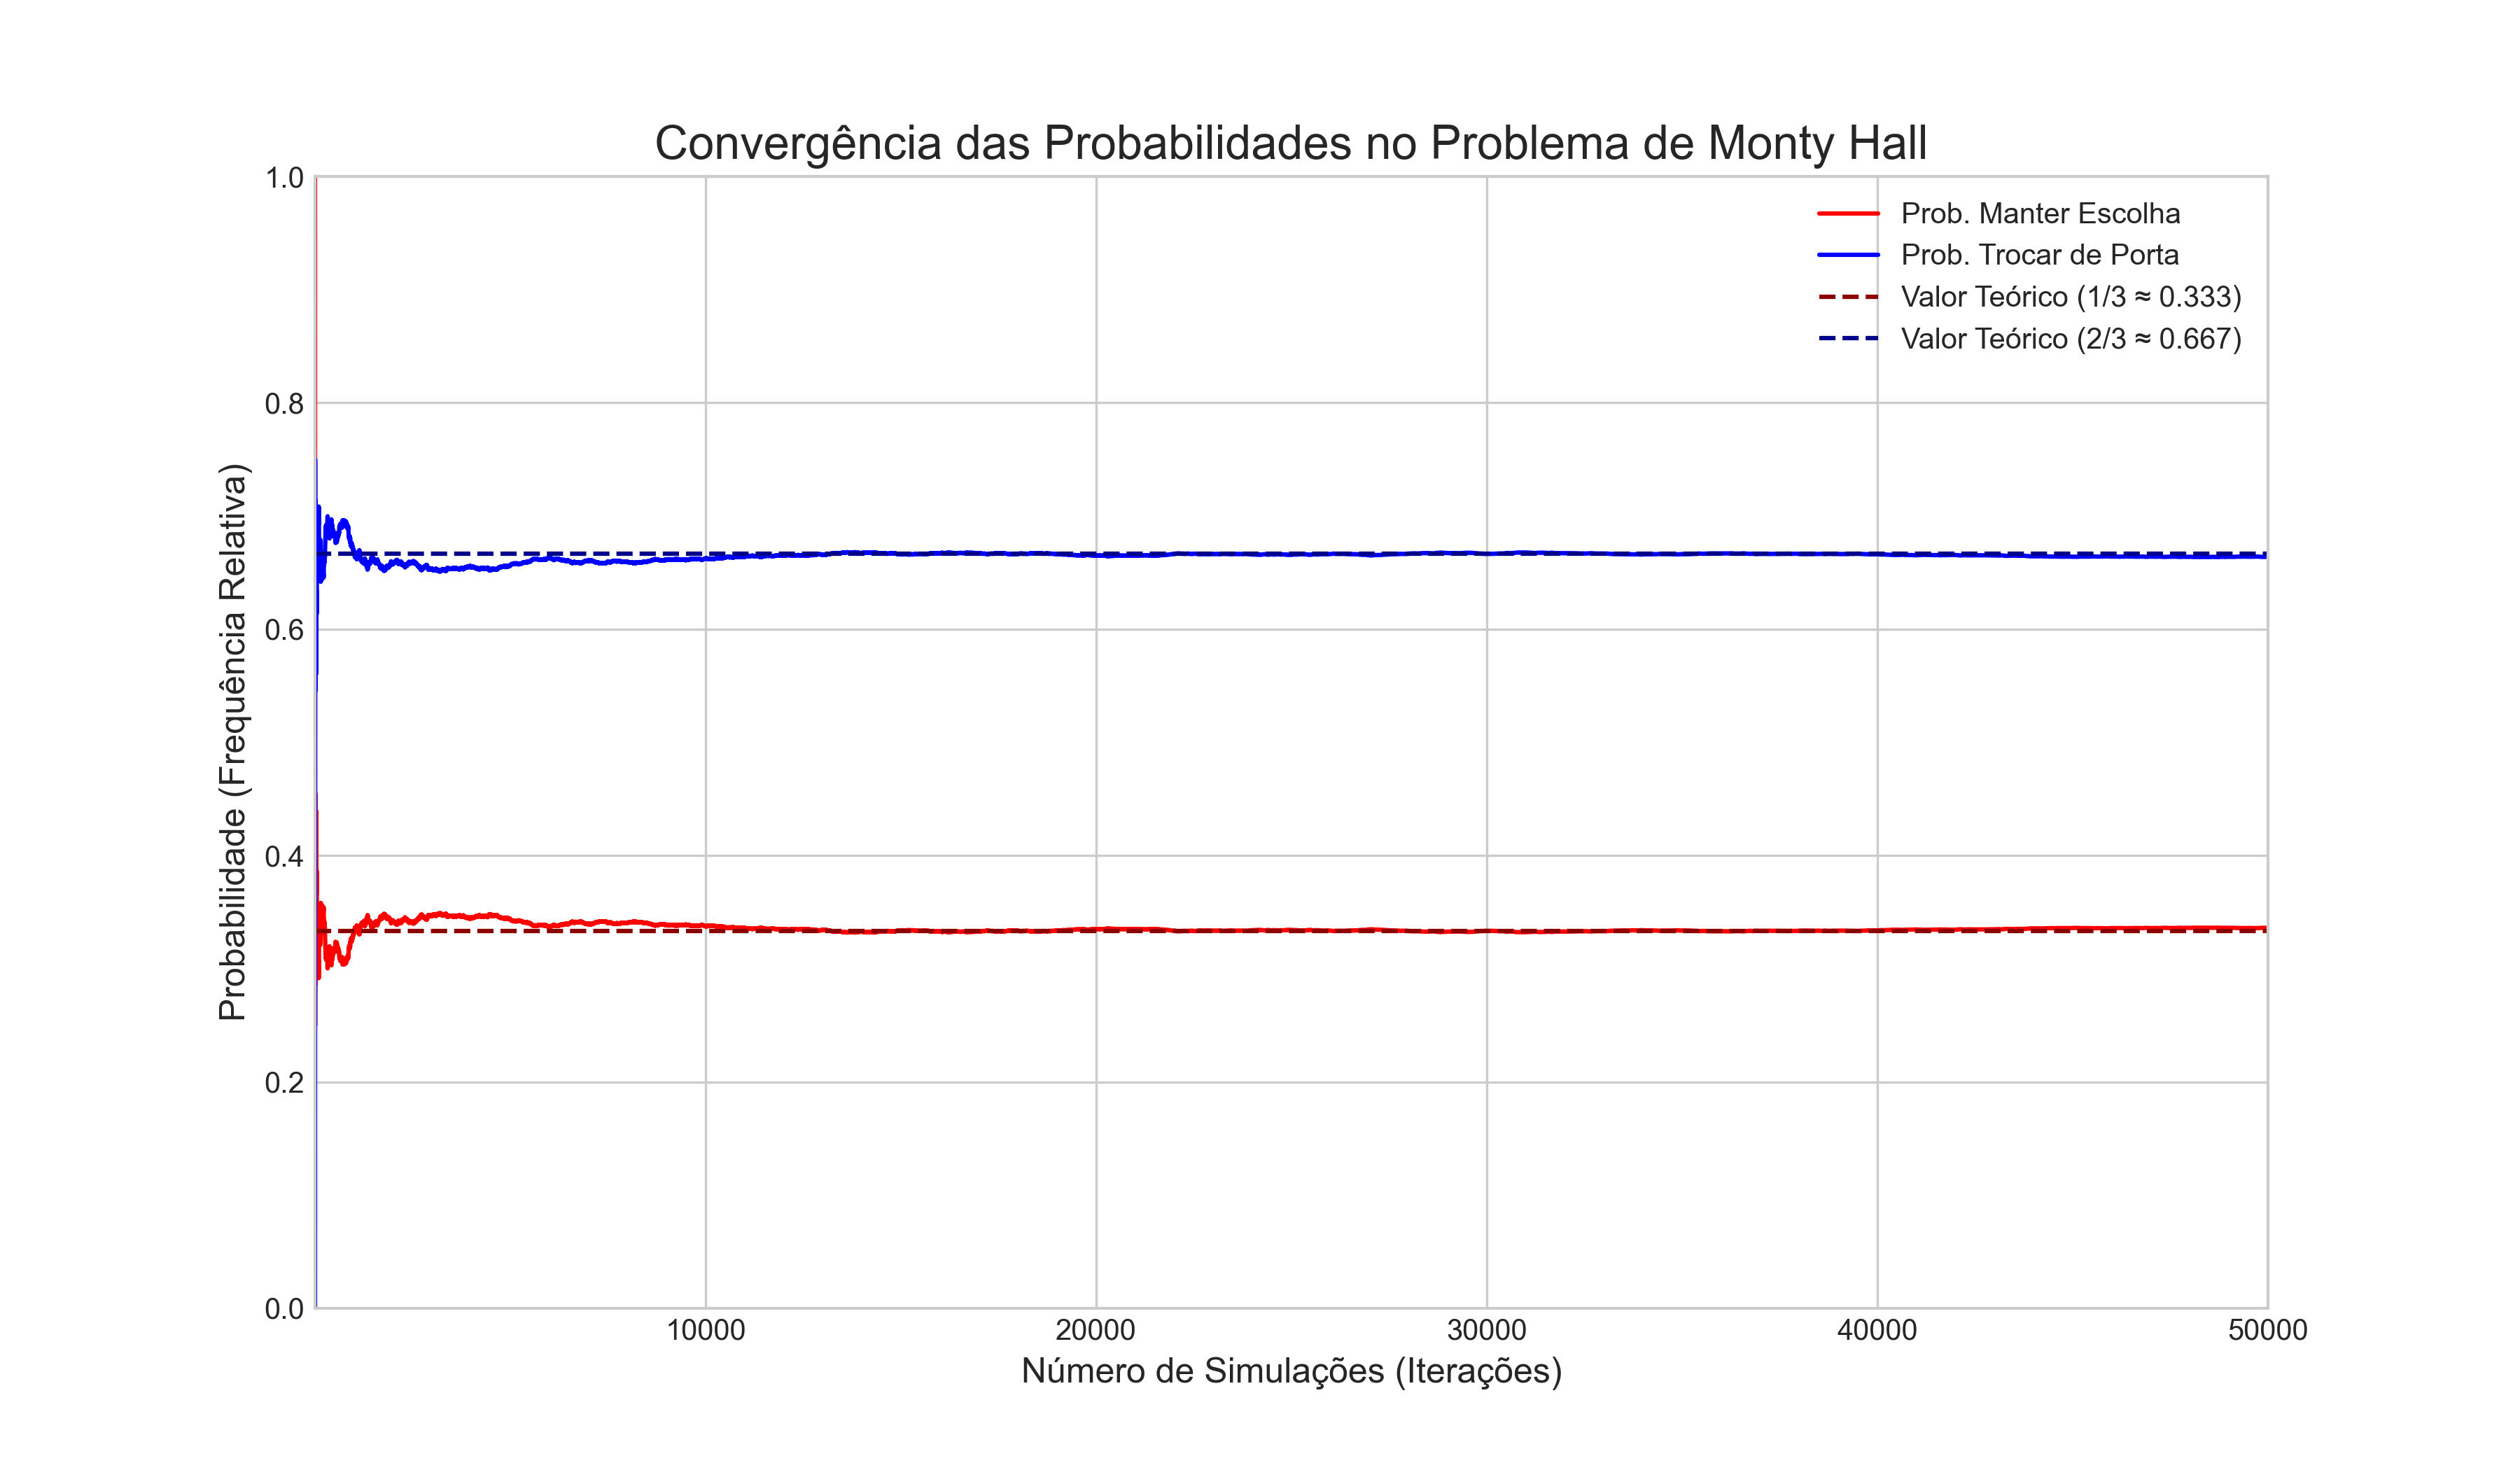
\includegraphics[width=0.9\linewidth]{figures/convergencia_monty_hall.png}
 \end{figure}
\end{frame}

% Slide 5: Código - Trocando
\begin{frame}[fragile]{Sempre trocando de porta}
A resposta intuitiva ao problema é a que quando o apresentador revelou uma das portas não premiadas, o participante passaria a ter um novo dilema com duas portas e um prêmio. Portanto, a chance do prêmio estar em uma das portas seria 1/2. 
 
A resposta contra-intuitiva e certa é que é mais vantajoso trocar, pois a
chance de ganhar trocando é o dobro da chance de ganhar sem trocar
\begin{figure}
    \centering
    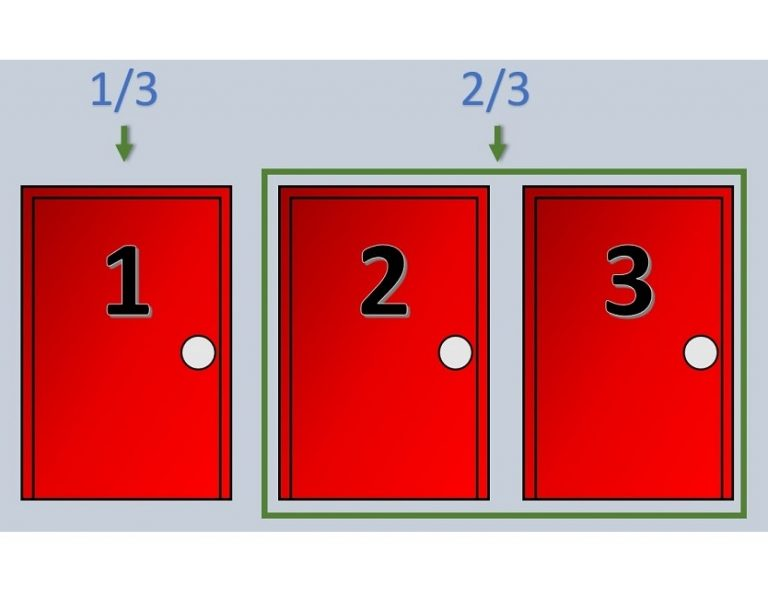
\includegraphics[width=0.45\linewidth]{figures/porc portas.jpg}
    \label{fig:enter-label}
 \end{figure}
\end{frame}

% Slide 6: Resultado
\begin{frame}{Solução}
\textbf{Resposta correta: é melhor trocar de porta!}

\vspace{0.3cm}
\begin{itemize}
  \item Probabilidade de ganhar sem trocar: \textbf{1/3}
  \item Probabilidade de ganhar trocando: \textbf{2/3}
\end{itemize}

\vspace{0.4cm}
\centering
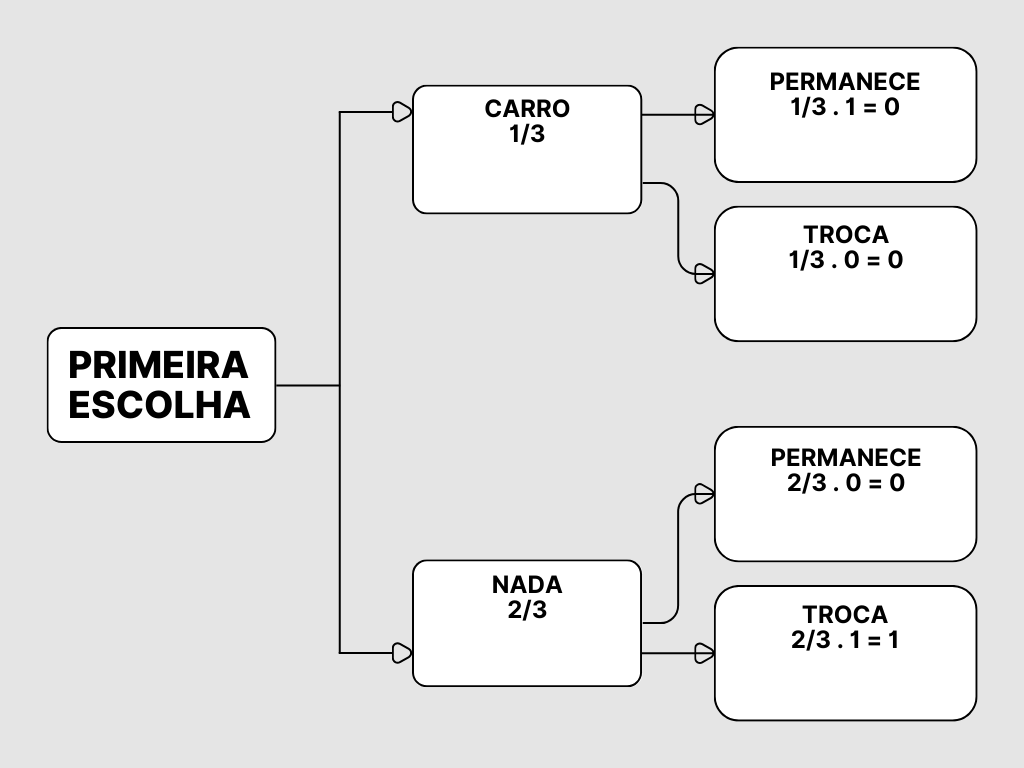
\includegraphics[width=0.4\textwidth]{figures/Grey and White Minimalist Simple Concept Map.png} 
\end{frame}